\section{Implementing \ac{pimc}}
\label{sec:implementing}

After thoroughly analysing state-of-the-art techniques to solve imperfect information games, and considering \emph{Sueca} is, at this moment, computationally unsolved, the chosen approach was \ac{pimc}.
Other presented techniques require computations that would be impractical to do at runtime, and therefore \ac{pimc} provide the best trade-off between computational resources and results for similar domains.

\begin{figure}[h!]
  \centering
    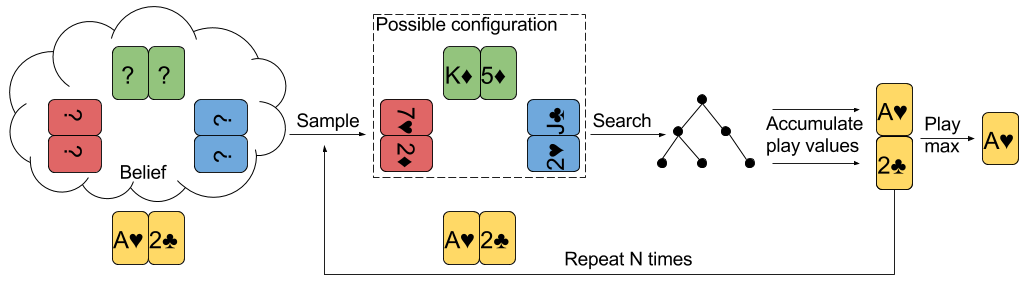
\includegraphics[width=1\textwidth]{./img/4/PIMC}
  \caption{\ac{pimc} algorithm illustrated to exemplify the choosing procedure in the 8\textsuperscript{th} trick}
\label{fig:PIMC}
\end{figure}

This algorithm samples cards distributions or configurations for other players' unknown hands.
Then, it calculates the reward of playing each card in its own hand for every sampled distribution.
The chosen card to play is, therefore, the one with the maximum accumulated reward for all the sampled distributions.

To implement this search technique, there are three key concepts or algorithms that require a full understanding: the Information Set, the \ac{pimc} and the MinMax Algorithm.
Moreover, the encountered drawbacks are also further described, as well as implemented enhancements to overcome those limitations.


\subsection{Information Set}
An information set represents all the visible information during a game, and also inferred information based on certain events.
The player must keep an instance of the information set per game and update it when necessary.
It stores the known hand of the player and a deck with all the cards whose owner is unknown.
As a result, each time another player plays a card, it should be removed from that deck.

The purpose of managing unplayed cards is to sample possible card distributions for the other three players with their real conditions.
These sampled distributions will be used during the \ac{pimc} search and the closer they are to the real world, the better the search returning value will be.
Additionally, the information set keeps track of suits per player and, when a player does not follow the leadsuit of a trick, it removes that suit from the player possible suits.
By possessing this information, sampling possible distributions gets even closer to the real world, however it increases the complexity of the sampling process.
The sampling method builds a \ac{csp} where:
\begin{itemize}
\item variables are the unplayed cards;
\item each domain is the set of players that still have that suit;
\item and the constraints are the number of times a player can be assigned to a card.
\end{itemize}


\subsection{\ac{pimc} Search}
The following pseudo-code of the \ac{pimc} search algorithm guided the implementation.

\begin{algorithm}
	\caption{PIMC search algorithm}
	\begin{algorithmic}[1]
		\Procedure{PIMC}{InfoSet $I$, int $N$}
			\ForAll {$m \in$ Moves($I$)}
				\State $val[m]$ = 0
			\EndFor
			\ForAll {$i \in \{ 1..N\}$}
				\State $x$ = Sample($I$)
				\ForAll {$m \in$ Moves($I$)}
					\State $val[m]$ += PerfInfoValue($x$, $m$)
				\EndFor
			\EndFor
			\State \textbf{return} $\underset{m}{argmax}\{ val[m] \}$
		\EndProcedure
		\label{alg:pimc}
	\end{algorithmic}
\end{algorithm}

To recapitulate the main points of this algorithm, considering it can choose up to \#Moves($I$), it samples $N$ possible card distributions for the other three players and calculates the reward of playing each possible move for the $N$ sampled worlds.
The returned move is the one that gave more accumulated reward.

The number of iterations this algorithm perform is imposed by the $N$ parameter.
Another version of the algorithm, instead of limiting the number of iterations, specifies the execution time of the main loop.


\subsection{MinMax Algorithm}
As mentioned above, \ac{pimc} has to calculate the reward of playing a card, for each sampled world (line 7 of Algorithm~\ref{alg:pimc}).
Since a sampled distribution assigns the remaining cards to players, every game can be handled as a perfect information game.
Therefore, to compute a perfect information game, considering each player or team intends to win, the MinMax algorithm was used.

MinMax is a popular algorithm for calculating optimal decisions in multiplayer games.
Each node corresponds to a possible move by a player and their successors correspond to the possible moves of the next player.
The player representing the agent and his team mate are both \emph{max} players, likewise, the other two opponents are \emph{min} players.

The complete game tree has 40 levels, from $l_{0}$ to $l_{39}$, and each group of $l_{4n}$ to $l_{4n+3}$ represents a trick.
Additionally, since the utility value can only be determined in terminal nodes, these back-propagate their best or worst child utilities, if they are \emph{max} or \emph{min} nodes, respectively.
The utility function to evaluate a sequence of moves deserved a serious consideration and is further detailed in Section~\ref{sec:parametrizing}.


\subsection{Drawbacks and enhancements}
When applying \ac{pimc} to decide which move \emph{m} to make, the number of computed game trees is \#Moves($I$) times $N$ (the number of different distributions), and the size of each game tree depends on the moves that are left to finish the game.
Additionally, the algorithm tends to choose a near optimal decision as long as the $N$ is reasonably large.
As a result, this algorithm has to process a large number of nodes to make a proper decision, specially in the beginning of the game, and, without the enhancements further described, this task was impractical.

\citet*{Russell2009} suggest that MinMax performance can be improved using alpha-beta prunning, a move ordering heuristic, and a transposition table.
Alpha-beta prunning, by simply storing the best choices so far for the max and min nodes, does not explore nodes that will not influence the final decision.

This technique can also be improved with a favourable ordering heuristic that produces earlier alpha-beta cuts.
Therefore, the implemented ordering heuristic is dynamic and uses an auxiliary computation to decide how to order moves.
Similarly to a human player reasoning, it analyses the current trick and tries to anticipate its winner.
If this auxiliary procedure expects the winner to be one of its opponents, it orders the cards from the less valuable to the most valuable, otherwise, it does the opposite.
This concept might bring a trade-off between the produced speed and the time spent on this extra computation plus the sort.
However, alpha-beta cuts have reasonably increased and, therefore, significantly reducing the exploration time of the whole tree.
\todo[inline]{Se houver tempo, quantificar a perfomance atingida com esta heuristica. FOI BRUTAL!}

Another improvement with remarkable results on the MinMax performance was a transposition table.
Considering each card configuration or distribution will produce \#Moves($I$) game trees, they will contain sufficient similar subtrees to store their first computed values.
Therefore, instead of recomputing them, they can be reused.
\todo[inline]{Detail time versus space problems. Too many days wasted on that deserves it!}

Furthermore, another heuristic was used, aiming to reduce redundancy in the state generation, suggested by \citet{Buro}.
When computing Moves($I$), two or more cards of the same suit, with consecutive ranks and with the same value can be considered as the same move, since they produce the same value.
For instance, holding 3$\clubsuit$, 4$\clubsuit$ and 5$\clubsuit$ on the same hand will produce three equivalent states and therefore, this heuristic produce only one.

Limiting the maximum depth achieved by the MinMax algorithm was another available option, specially for earlier decisions that produce larger trees and the time to compute them was impractical.
However, considering a non-terminal node as terminal may imply the utility function to be revised or somehow predicted.
Different parametrizations related to the depth cut are detailed further in Section~\ref{sec:parametrizing}

%Lastly, to exploit the computational resources and considering the fact that \ac{pimc} can be easily paralleled, the outer loop was divided into the number of \acp{cpu} the machine has.
%Using a machine with 4 \acp{cpu}, the speed-up is nearly 4.
%The only concern while paralleling this algorithm is to carefully manage the scope of shared and private variables among the threads.











